%% LyX 2.2.3 created this file.  For more info, see http://www.lyx.org/.
%% Do not edit unless you really know what you are doing.
\documentclass[10pt,english]{article}
\usepackage[T1]{fontenc}
\usepackage[latin9]{inputenc}
\usepackage{geometry}
\geometry{verbose,tmargin=2cm,bmargin=2cm,lmargin=2cm,rmargin=2cm,headheight=2cm,headsep=2cm,footskip=1cm}
\usepackage{babel}
\usepackage{float}
\usepackage{graphicx}
\PassOptionsToPackage{normalem}{ulem}
\usepackage{ulem}
\usepackage[unicode=true]
 {hyperref}
\begin{document}

\title{Lightweight Publish-Subscribe Application Protocol}

\author{Matteo M. Fusi, Paolo Mosca}

\maketitle
\tableofcontents{}

\pagebreak{}

\section{Introduction and General Informations}

\subsection{Purpose of the Document}

This document is part of the project of the \emph{Internet of Things
}course at Politecnico di Milano for the Academic Year 2016/2017.
This document is associated to the source code at the link \href{https://github.com/fusiled/tinyos-simple-mqtt}{https://github.com/fusiled/tinyos-simple-mqtt}.

\subsection{Essential Informations}

The project is written with the TinyOS framework. We developed two
kinds of nodes that must be run in Cooja simulation environment: \textbf{\emph{PanC}}\emph{
}is the PAN Coordinator and \textbf{\emph{NodeC}} is responsbile of
collecting measurements and sending them to the PAN Coordinator. \emph{NodeC
}components can send/receive messages to/from \emph{PanC}. There can
be only one \emph{PanC }in the network and up to 8 \emph{NodeC }components.
How the two components are wired and structured is described in the
section named \emph{Description of the Components}.

\subsubsection{\emph{TOS\_NODE\_ID and Address Layout}}

\emph{PanC }\uline{must} have \emph{ActiveMessageAddressC\_\_addr
}set to 9. \emph{NodeC }components rely on this information when they
have someting to send. \emph{TOS\_NODE\_ID} can have any value $\geq8$.
\emph{NodeC }components has a \emph{TOS\_NODE\_ID} in the range $[1;8]$
and they have \emph{ActiveMessageAddressC\_\_addr }equal\emph{ to
TOS\_NODE\_ID. }Every message has a \emph{node\_id }field attached
to it and the meaning changes on the message\_type (See \emph{Layout
of the Messages }for further details). \emph{node\_id }is set in messages
as \emph{TOS\_NODE\_ID-1. }With this method it is possible to save
1 bit in the \emph{node\_id }field of the messages. The method of
how to properly set the \emph{TOS\_NODE\_ID }symbols is described
in \emph{Simulation Environment} section. 

\section{Description of the Components}

There are two approaches to handle messages: one it is based on timeout
and it's used with \emph{connect/connack }and \emph{subscribe/suback}
messages and the other uses a resend buffer when a send fails for
some reason. The first method is ok for simple send-and-ack messages
(like, in fact, connect and subscribe message sequences): we don't
have any kind of timing constraints, so it's tolerable to connect
a node not immediatly or know which topics a node is interested. What
we wanted was to ensure that informations (the measurements) arrived
at their destination, because they're the most important data in the
network. That's why we implemented the resend buffer: to ensure that
surely \emph{publish }messages will arrive to thei destination.

\subsection{Node}

A Node can send only \emph{connect,subscribe,publish }and \emph{puback
}messages. For the sake of simplicity, interested topics and QOS of
the topics are hardcoded and are based on the \emph{NODE\_ID }of the
node.

\paragraph{The State Machine}

A node has a state variable (called \emph{state}) which controls the
behaviour of the component. If \emph{state }is set to:
\begin{description}
\item [{\emph{NODE\_STATE\_CONNECTING}}] The node can only try to connect
to PAN Coordinator. Other operations are not possible
\item [{\emph{NODE\_STATE\_SUBSCRIBING}}] The node has received \emph{connack.
}Now it's sending the \emph{subscribe }message and/or is waiting for
the \emph{suback. }In this state the node can collect measurements
and publish them.
\item [{\emph{NODE\_STATE\_PUBLISHING}}] The node has received the \emph{suback.
}The node now must only collect and publish measurements.
\end{description}
The behaviour is briefly explained by the following finite state machine:
\begin{figure}[h]
\begin{centering}
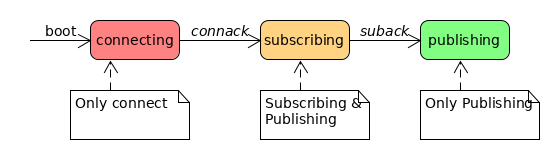
\includegraphics[width=8cm]{img/node_state_diagram}
\par\end{centering}
\caption{Control State Machine of a Node}

\end{figure}
.

\paragraph{\emph{connect }and \emph{subscribe }handling}

These two messages are controlled by a timeout timer: when there's
an attempt to send one of these messages a timer is started. If i
don't receive the realted ack (a \emph{connack }or a \emph{suback})\emph{,
}then the node will try to send another message of the same kind.
Note that \emph{PacketAcknowledgment.requestAck }call is not needed.

\paragraph{\emph{publish }and \emph{puback} handling}

They use a different mechanism: at first there's an attempt to send
the message, if the sending procedure fails for some reason (the network
component is busy or the ack set by the \emph{PacketAcknowledgment
}interface is not received when QOS=1), then the message is stored
into a resend buffer that it's a simple queue. This resend buffer
try to send a message every \emph{RESEND\_DELTA\_TIME }milliseconds\emph{.
}If the buffer is full then a packet is discarded, so it's important
that the parameters of the buffer are well-sized. If the resend buffer
fails to send a message, then this message is put at the tail of the
queue.

\paragraph{Collecting measurements and sending them}

The node implements a timer which triggers periodically every \emph{SENSOR\_PERIOD}
seconds. When the time triggers one of the three sensors is selected
and the related command needed to fetch the measurement is called.
The three possible type of measurements are temperature, humidity
and luminosity.
\begin{figure}[H]
\begin{centering}
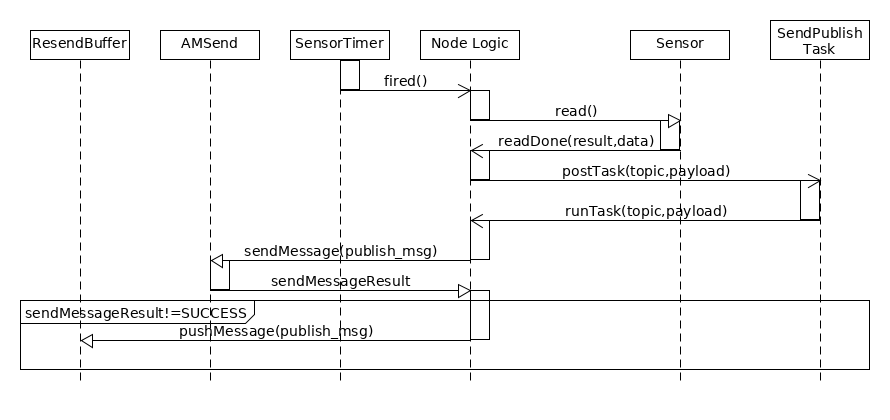
\includegraphics[width=14cm]{img/sensor_read}
\par\end{centering}
\caption{Sequence Diagram of the Collection and Sending of a measurement}

\end{figure}

\subsection{PAN Coordinator}

PAN Coordinator is a passive agent because it acts only when it receive
a message.

\paragraph{\emph{connect }and \emph{subscribe }handling}

When the PAN Coordinator receives a \emph{connect }it marks the node
who sent the \emph{connect }as active (it keeps an array of boolean
to keep the in memory the state of every node) and replies with a
\emph{connack}. The same methodolgy is used with \emph{subscribe }messages
but the node saves the topic in which a node is interested and the
associated QOSs. The peculiarity is that the PAN Coordinator acts
lazy when it must reply to\emph{ connect }and \emph{subscribe }messages:
if the PAN Coordinator can't send \emph{connack }or \emph{suback }the
it just fails and it will do nothing. The PAN Coordinator will try
to resend another \emph{connack }or \emph{suback }when the node who
has not received the associated ack message will resend the \emph{connect
}or the \emph{subscribe} because the timeout associated is expired.

\paragraph{\emph{publish }and \emph{puback }handling}

When the PAN Coordinator receives a \emph{publish} it replies immediatly
with e \emph{puback }and it forward the \emph{publish }to all the
interested nodes. It uses \emph{PacketAcknowledgment.requestAck }in
case the destination of the nodes required QOS=1 for the topic of
the inquiring \emph{publish}. If one of the messages cited fails then
it is put in a resend buffer which acts exactly like described in
the Node section: it tries to send the element in its queue every
\emph{RESEND\_DELTA\_TIME }milliseconds. \emph{PacketAcknowledgment.requestAck
}in case QOS=1 guarantees that the packets are received by the destination
node and the mechanism helps to know if we must retransmit the message
without complex mechanism: if the ack is not received, then resend.

\section{Messages}

\subsection{Layout of the Messages}

The messages have been designed in order to be as small as possible.
The structures and the functions realted to messages are contained
in the source file \emph{commons/Commons.h. }What and when a message
is sent is descibed in the section named \emph{The Implemented Publish-Subscribe
Mechanism}. Two fields are common in every type of message and their
size and positioning in the message layout is fixed:
\begin{description}
\item [{code\_id}] It is a 3bit field. It occupies the 3 less significant
bits. This field contains a code that identifies the message.
\item [{node\_id}] It is a 3bit filed. It occupied the 3 less significant
bts after the \emph{code\_id }field. This filed contains a node\_id.
It is usually identifies the source of a message if sent from a \emph{NodeC
}components. If a message is sent from the \emph{PanC }module, then
it identifies the destination of the message, but when the mesaage
is a publish then it contains the id of the node who published.
\end{description}

\paragraph{CONNECT}

The \emph{code\_id }is\emph{ 1. }It is 8 bits big. It has not any
other field other than \emph{node\_id }and \emph{code\_id. }The \emph{node\_id
}tells to then PAN Coordinator which node requested a connection.

\paragraph{CONNACK}

The \emph{code\_id }is\emph{ 2. }It is 8 bits big. It has not any
other field other than \emph{node\_id }and \emph{code\_id. }The \emph{node\_id
}tells to which node the \emph{connack }message is destined.

\paragraph{PUBLISH}

The \emph{code\_id }is\emph{ 3. }It is 32 bits big. The other fields
after \emph{node\_id }and \emph{code\_id }are\emph{:}
\begin{description}
\item [{\emph{publish\_topic}}] This field is 2 bits big. It identifies
the topic of the publish: 0 is temperature, 1 is humidity and 2 is
luminosity.
\item [{\emph{publish\_id}}] This field is 8 bits big. It uniquely identify
a publish. The range of the ids is limited, but we assume that it's
not possible that there are in the network 2 messages with the same
id at the same time. This id is used to match \emph{publish }with
related \emph{puback }messages.
\item [{\emph{publish\_qos}}] This field is 1 bit big. If the source of
the message is \emph{NodeC}, then it tells to PAN Coordinator if send
a \emph{puback }or not. If the source of the message is \emph{PanC},
then it is the qos related to \emph{publish\_topic }of the destination
\emph{NodeC }specified previously int the \emph{subscribe }message.
\item [{\emph{publish\_payload}}] This field is 15 bits big. It's the value
of the collected measure.
\end{description}

\paragraph{PUBACK}

The \emph{code\_id }is\emph{ 4. }It is 16 bits big. The other fields
after \emph{node\_id }and \emph{code\_id }are\emph{:}
\begin{description}
\item [{\emph{puback\_topic}}] This field is 2 bits big. This field contains
the topic associated to the related \emph{publish }message.
\item [{\emph{puback\_publish\_id}}] This field is 8 bits big. This id
is used to match \emph{publish }with related \emph{puback }messages.
\end{description}

\paragraph{SUBSCRIBE}

The \emph{code\_id }is\emph{ 5. }It is 16 bits big. The other fields
after \emph{node\_id }and \emph{code\_id }are\emph{:}
\begin{description}
\item [{\emph{topic\_mask}}] This field is 3 bits big. This is mask tells
to PAN Coordinator if the source of the message is interested or not
into a specific topic. The least significant bit is associated to
temperature, the second least significant bit is associated to humidity
and the remaining bit is associated to luminosity. If a bit has value
0, then the node is not interested into a topic, otherwise yes.
\item [{\emph{qos\_mask}}] This field is 3 bits big. It is composed exactly
as the \emph{topic\_mask }field, but it expresses how the PAN Coordinator
must behave when it sends a \emph{publish }to the inquiring node.
\end{description}

\paragraph{SUBACK}

The \emph{code\_id }is\emph{ 6. }It is 8 bits big. It has not any
other field other than \emph{node\_id }and \emph{code\_id. }The \emph{node\_id
}tells to which node the \emph{suback }message is destined.
\end{document}
